\section{Comparative Evaluation and Analysis}
\label{sec:experiments}

We evaluate our proposed framework through a series of comparative experiments designed to identify the optimal architecture and representation for bimanual garment folding. Table \ref{tab:per_garment_results} presents the results for all of our primary experiments, while Figure \ref{fig:qualitative_results} provides visual snapshots of successful and failed folding sequences across different categories for our best model. Our evaluation follows a three-phase journey, moving from baseline diffusion models to large-scale VLAs, and finally to optimized action chunking.

\subsection{Diffusion Policy}
Our initial experiments utilized Diffusion Policy (DP) \cite{chi2023diffusionpolicy}. As shown in Table \ref{tab:per_garment_results}, DP achieved a macro-average success rate of only 11.67\%. While it showed some capability in the "Pant Short" category (38.33\%), it failed almost entirely on tops. Qualitative analysis revealed that DP struggled with the high-precision coordination required for bimanual folding; the two arms often produced inconsistent joint targets, leading to garment entanglement.

\subsection{Vision-Language-Action Models}
To leverage semantic priors, we transitioned to Vision-Language-Action (VLA) models. We evaluated SmolVLA \cite{smolvla2025}, $\pi_{0.5}$ \cite{pi05_2026}, and X-VLA \cite{zheng2025xvlasoftpromptedtransformerscalable} with Low-Rank Adaptation (LoRA). Due to the high computational cost of fine-tuning large VLAs on a shared HPC environment, we decided to not evaluate all models on all garment categories if their initial results on a subset and subsequent video analysis showed inherent architectural limitations. 

\begin{figure*}[t]
    \centering
    \setlength{\tabcolsep}{1pt}
    \begin{tabular}{cccccccc}
        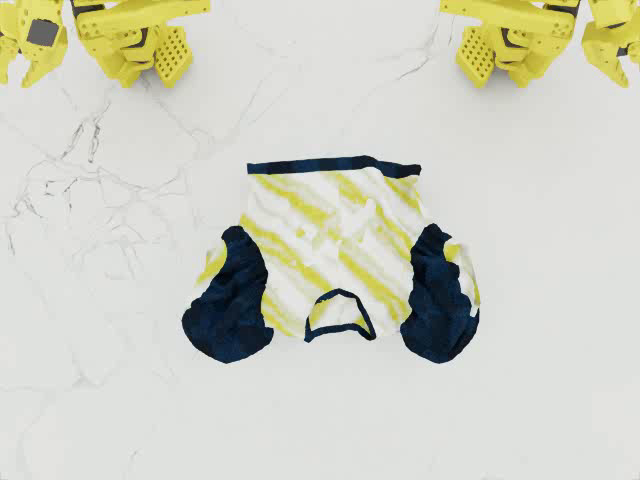
\includegraphics[width=0.12\textwidth]{fig/qualitative/pi05_failure_ext_0.png} &
        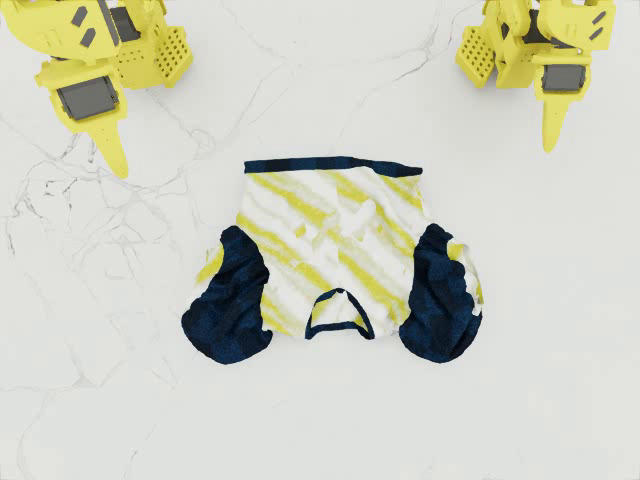
\includegraphics[width=0.12\textwidth]{fig/qualitative/pi05_failure_ext_1.png} &
        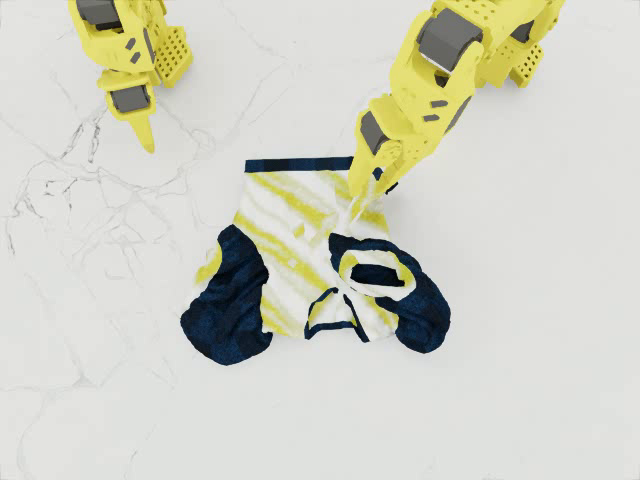
\includegraphics[width=0.12\textwidth]{fig/qualitative/pi05_failure_ext_2.png} &
        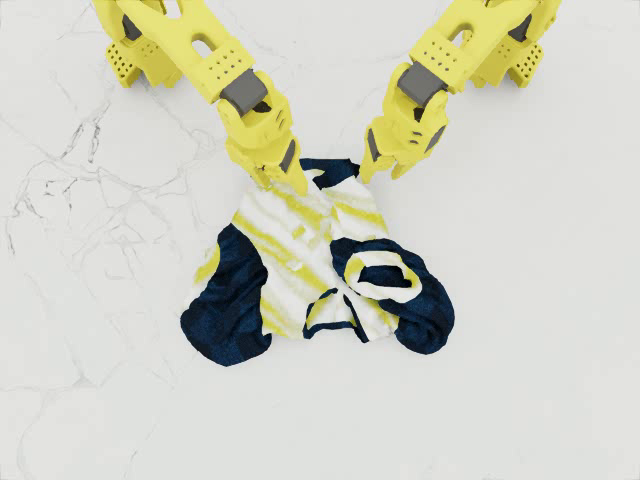
\includegraphics[width=0.12\textwidth]{fig/qualitative/pi05_failure_ext_3.png} &
        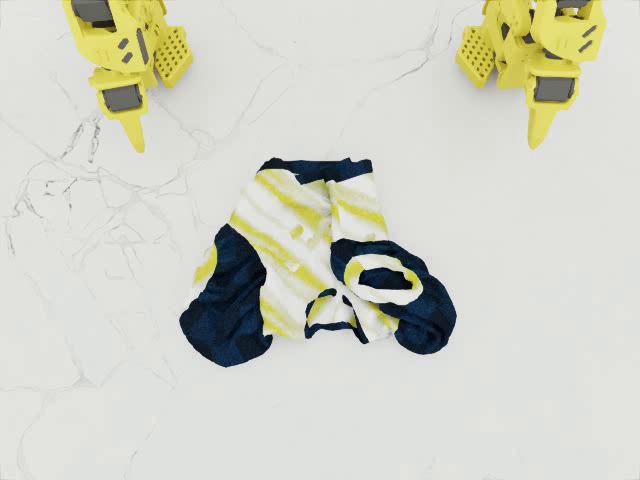
\includegraphics[width=0.12\textwidth]{fig/qualitative/pi05_failure_ext_4.png} &
        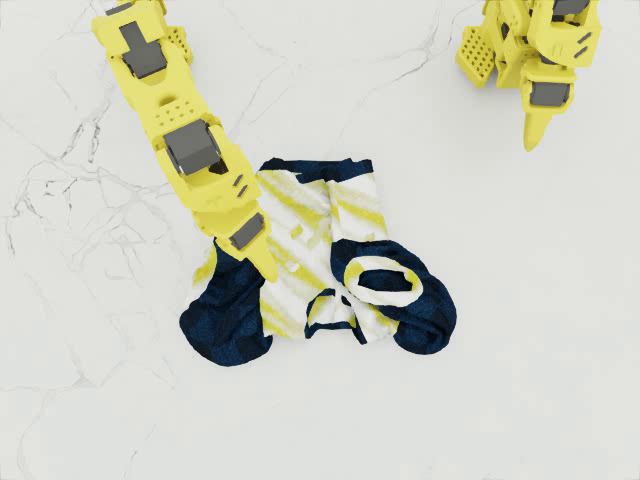
\includegraphics[width=0.12\textwidth]{fig/qualitative/pi05_failure_ext_5.png} &
        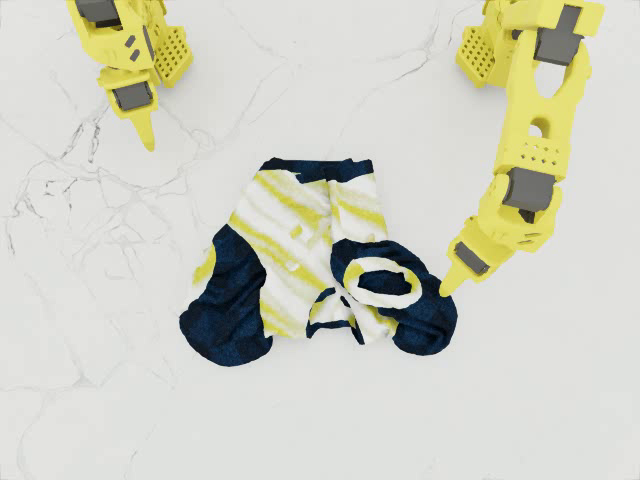
\includegraphics[width=0.12\textwidth]{fig/qualitative/pi05_failure_ext_6.png} &
        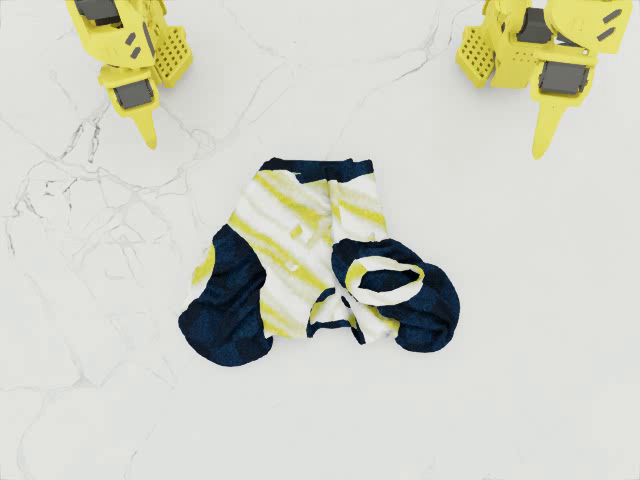
\includegraphics[width=0.12\textwidth]{fig/qualitative/pi05_failure_ext_7.png} \\
        \tiny $t=0.0s$ & \tiny $t=2.0s$ & \tiny $t=4.0s$ & \tiny $t=6.0s$ & \tiny $t=8.0s$ & \tiny $t=10.0s$ & \tiny $t=12.0s$ & \tiny $t=14.0s$ \\
        \multicolumn{8}{c}{\small (a) $\pi_{0.5}$ + PEFT: Erratic joint targets and failure to localize.} \\
        \vspace{4pt} \\
        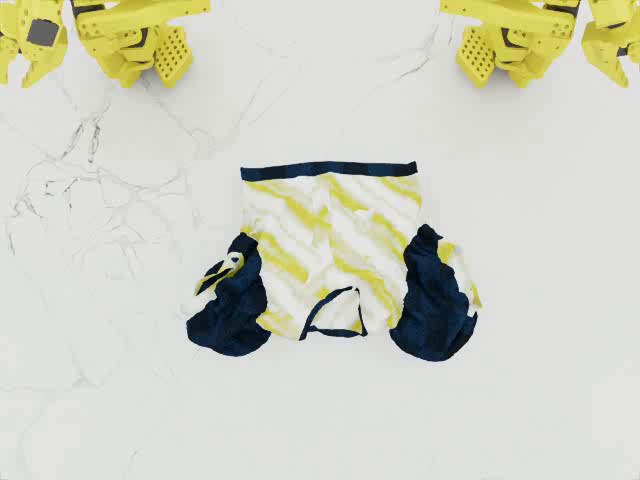
\includegraphics[width=0.12\textwidth]{fig/qualitative/xvla_failure_ext_0.png} &
        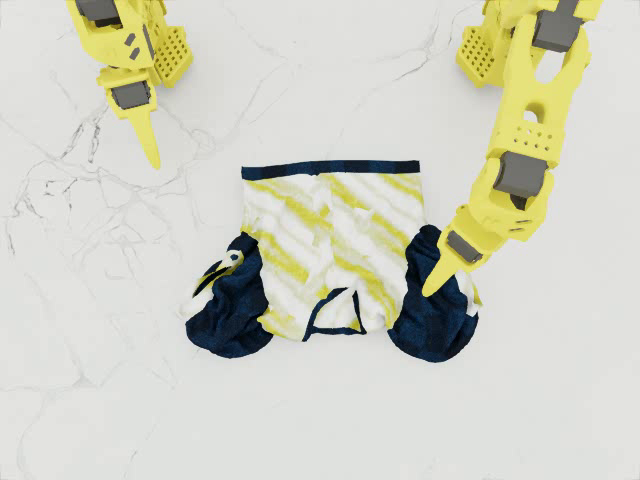
\includegraphics[width=0.12\textwidth]{fig/qualitative/xvla_failure_ext_1.png} &
        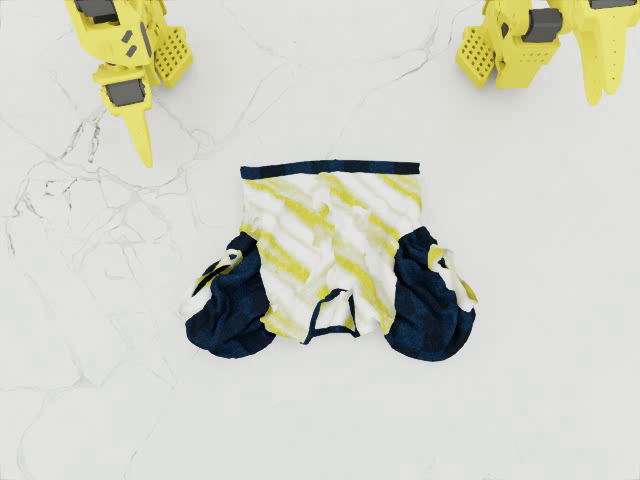
\includegraphics[width=0.12\textwidth]{fig/qualitative/xvla_failure_ext_2.png} &
        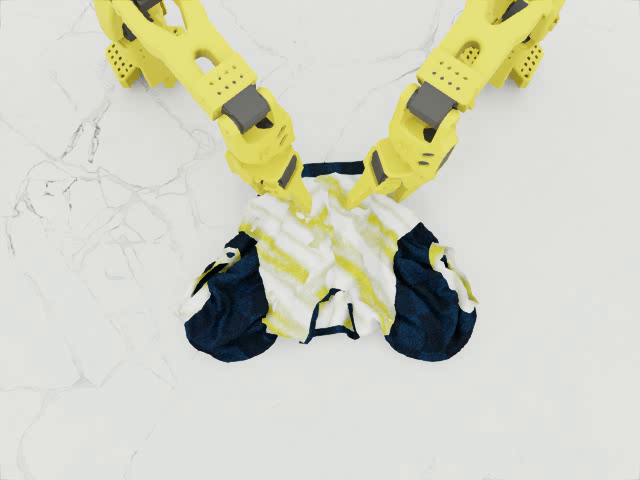
\includegraphics[width=0.12\textwidth]{fig/qualitative/xvla_failure_ext_3.png} &
        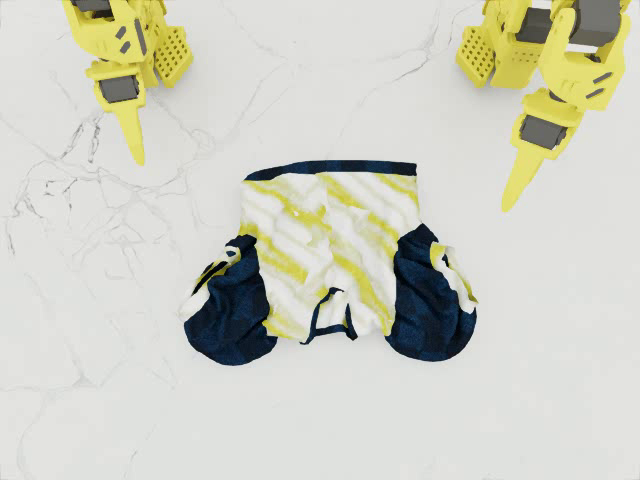
\includegraphics[width=0.12\textwidth]{fig/qualitative/xvla_failure_ext_4.png} &
        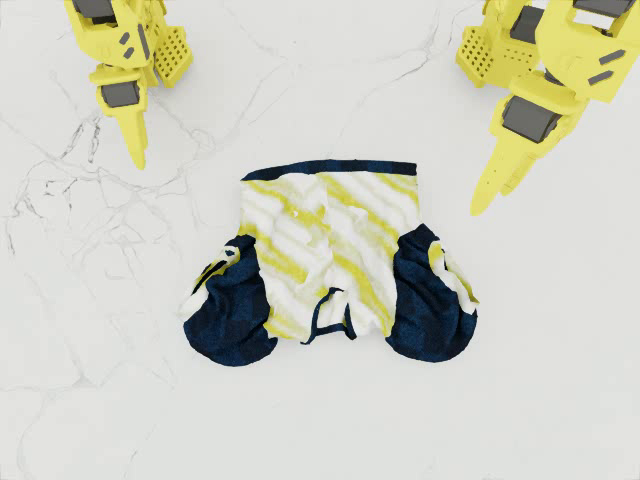
\includegraphics[width=0.12\textwidth]{fig/qualitative/xvla_failure_ext_5.png} &
        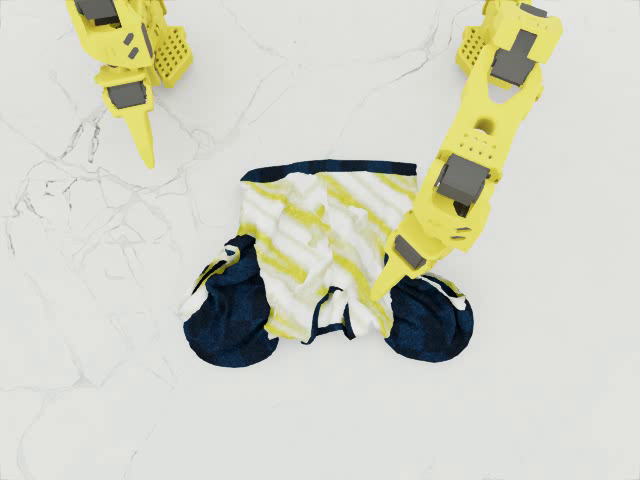
\includegraphics[width=0.12\textwidth]{fig/qualitative/xvla_failure_ext_6.png} &
        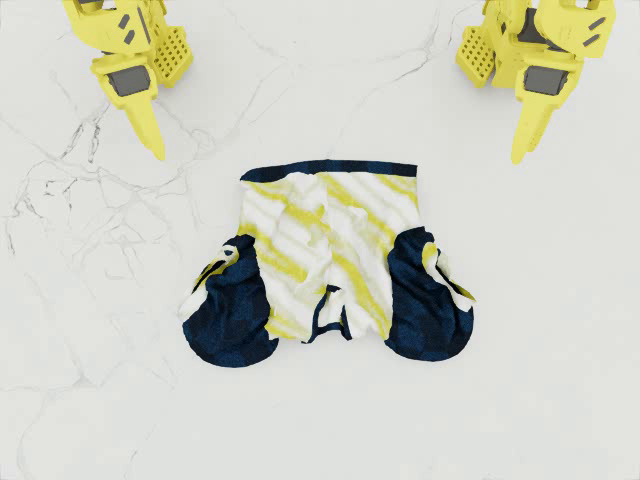
\includegraphics[width=0.12\textwidth]{fig/qualitative/xvla_failure_ext_7.png} \\
        \tiny $t=0.0s$ & \tiny $t=2.0s$ & \tiny $t=4.0s$ & \tiny $t=6.0s$ & \tiny $t=8.0s$ & \tiny $t=10.0s$ & \tiny $t=12.0s$ & \tiny $t=14.0s$ \\
        \multicolumn{8}{c}{\small (b) X-VLA: Gripper failure and lack of grasping initiation.} \\
    \end{tabular}
    \caption{Qualitative analysis of large-scale VLA failure modes. Unlike ACT, these models struggled with basic robotic control primitives, exhibiting high-frequency jitter and an inability to maintain contact with the cloth.}
    \label{fig:vla_failures}
\end{figure*}

As shown in Figure \ref{fig:vla_failures}, X-VLA and $\pi_{0.5}$ exhibited near-zero performance. X-VLA failed to even close its gripper (Figure \ref{fig:vla_failures}b), while $\pi_{0.5}$ struggled to localize the garment, often producing erratic and dangerous joint velocities (Figure \ref{fig:vla_failures}a). We attribute these failures to the limited scale of our demonstration dataset, which was insufficient for fine-tuning models of this magnitude. Notably, SmolVLA significantly outperformed these larger models, likely because its smaller parameter count (approx. 500M) made it more amenable to task-specific alignment in our low-data regime, whereas the massive capacity of the larger VLAs led to catastrophic control failures when forced to adapt to such a specialized domain.

\begin{figure*}[t]
    \centering
    \setlength{\tabcolsep}{1pt}
    \begin{tabular}{cccccccc}
        
\includegraphics[width=0.12\textwidth]{fig/qualitative/tl_success_0.png} &
        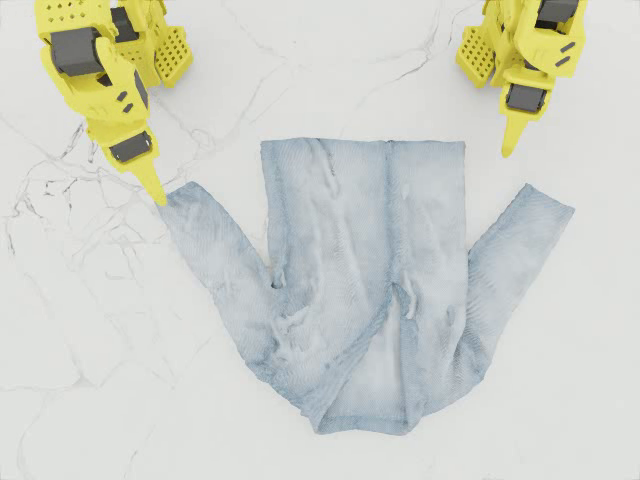
\includegraphics[width=0.12\textwidth]{fig/qualitative/tl_success_1.png} &
        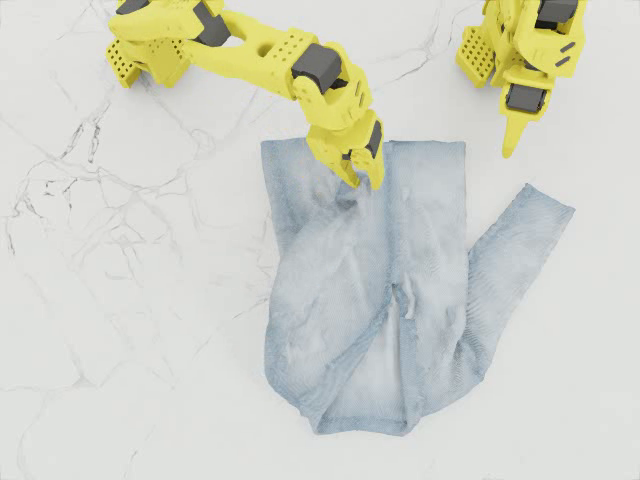
\includegraphics[width=0.12\textwidth]{fig/qualitative/tl_success_2.png} &
        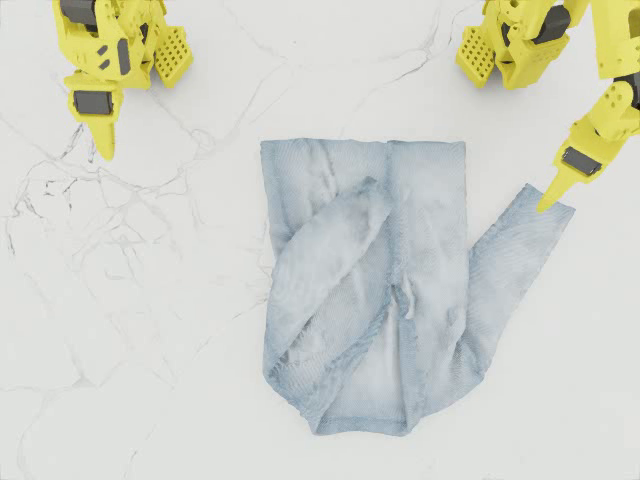
\includegraphics[width=0.12\textwidth]{fig/qualitative/tl_success_3.png} &
        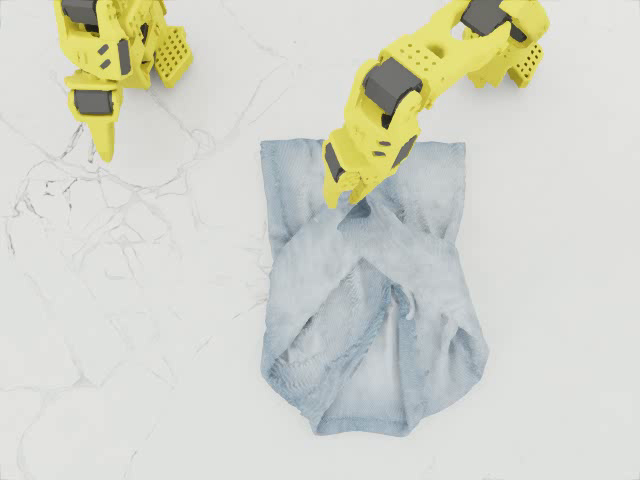
\includegraphics[width=0.12\textwidth]{fig/qualitative/tl_success_4.png} &
        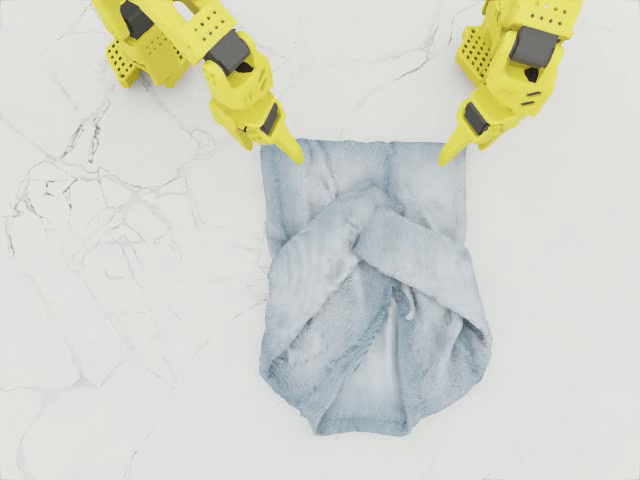
\includegraphics[width=0.12\textwidth]{fig/qualitative/tl_success_5.png} &
        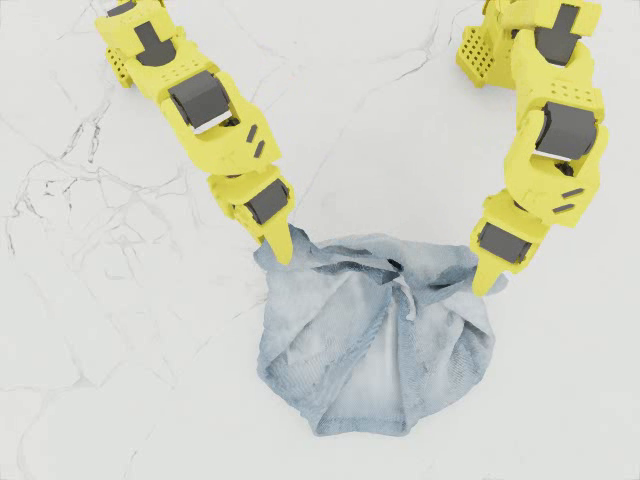
\includegraphics[width=0.12\textwidth]{fig/qualitative/tl_success_6.png} &
        
\includegraphics[width=0.12\textwidth]{fig/qualitative/tl_success_7.png} \\
        \tiny $t=0.0s$ & \tiny $t=1.5s$ & \tiny $t=3.0s$ & \tiny $t=4.5s$ & \tiny $t=6.0s$ & \tiny $t=7.5s$ & \tiny $t=9.0s$ & \tiny $t=10.5s$ \\
        \multicolumn{8}{c}{\small (a) Top-Long Success Sequence} \\
        \vspace{2pt} \\
        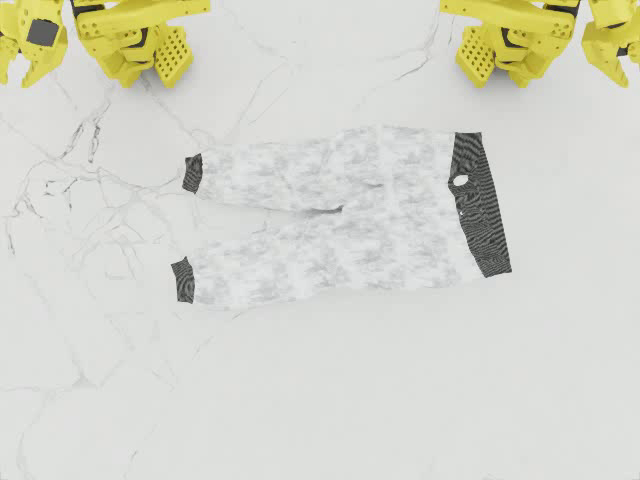
\includegraphics[width=0.12\textwidth]{fig/qualitative/pl_success_0.png} &
        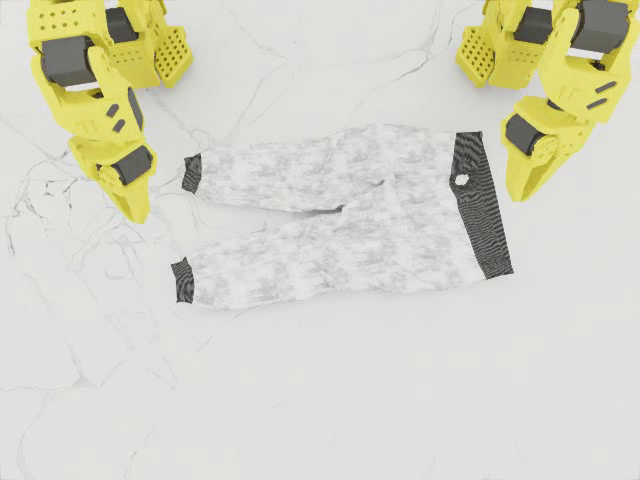
\includegraphics[width=0.12\textwidth]{fig/qualitative/pl_success_1.png} &
        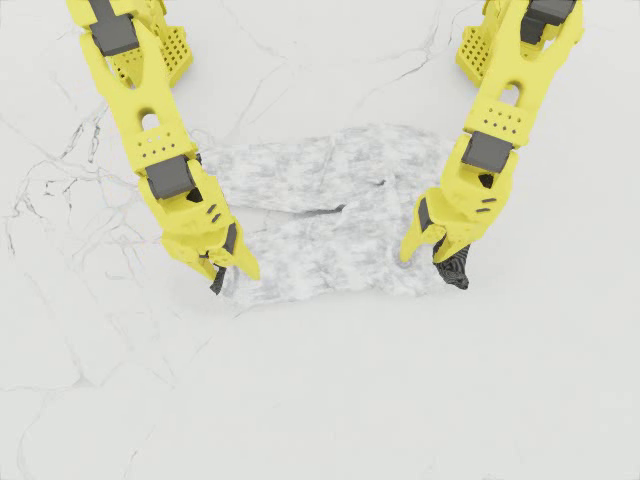
\includegraphics[width=0.12\textwidth]{fig/qualitative/pl_success_2.png} &
        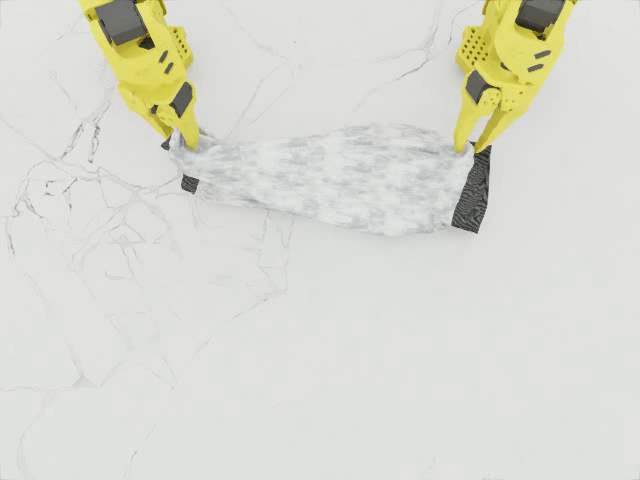
\includegraphics[width=0.12\textwidth]{fig/qualitative/pl_success_3.png} &
        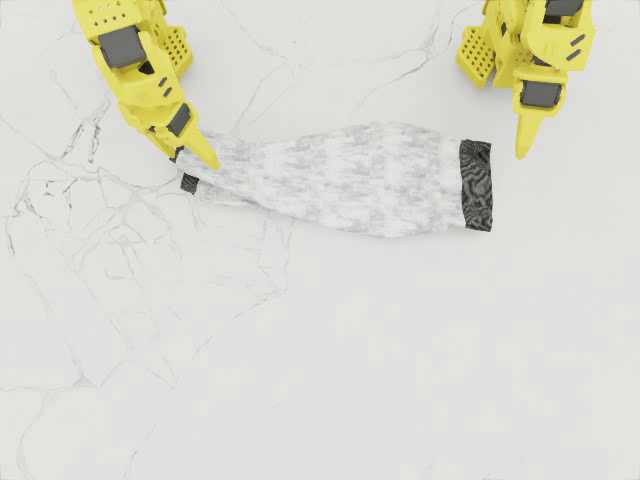
\includegraphics[width=0.12\textwidth]{fig/qualitative/pl_success_4.png} &
        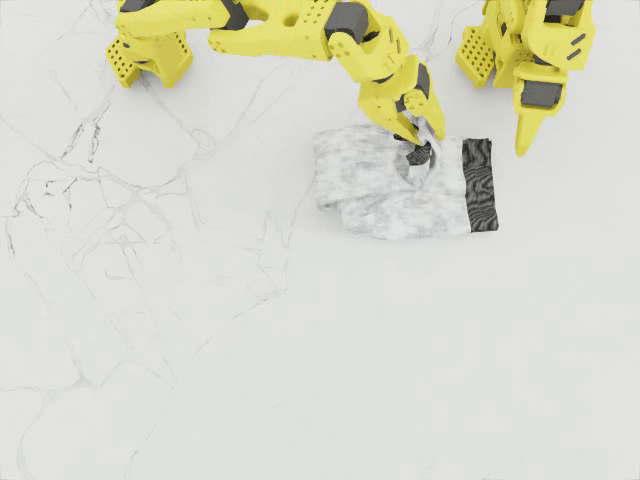
\includegraphics[width=0.12\textwidth]{fig/qualitative/pl_success_5.png} &
        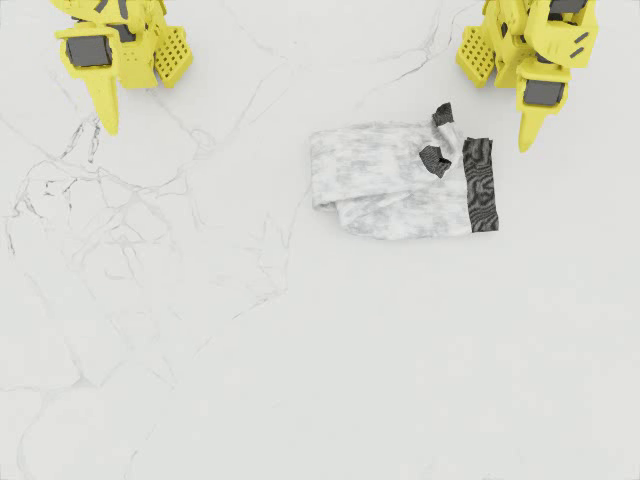
\includegraphics[width=0.12\textwidth]{fig/qualitative/pl_success_6.png} &
        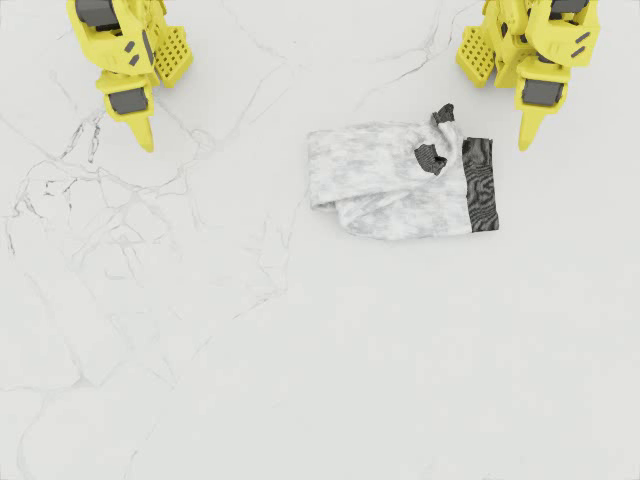
\includegraphics[width=0.12\textwidth]{fig/qualitative/pl_success_7.png} \\
        \tiny $t=0.0s$ & \tiny $t=1.5s$ & \tiny $t=3.0s$ & \tiny $t=4.5s$ & \tiny $t=6.0s$ & \tiny $t=7.5s$ & \tiny $t=9.0s$ & \tiny $t=10.5s$ \\
        \multicolumn{8}{c}{\small (b) Pant-Long Success Sequence} \\
        \vspace{2pt} \\
        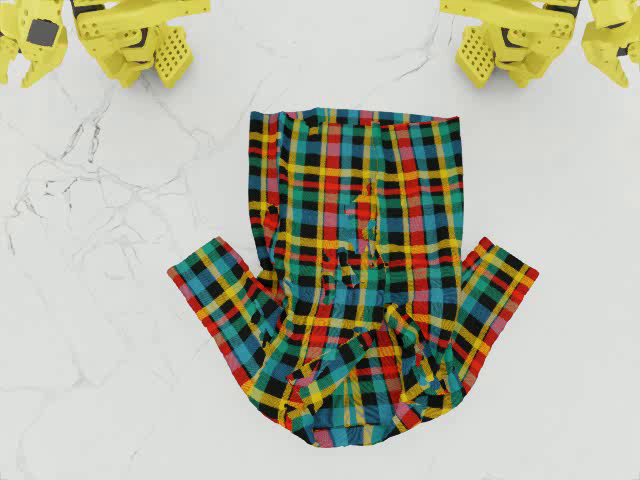
\includegraphics[width=0.12\textwidth]{fig/qualitative/ts_failure_0.png} &
        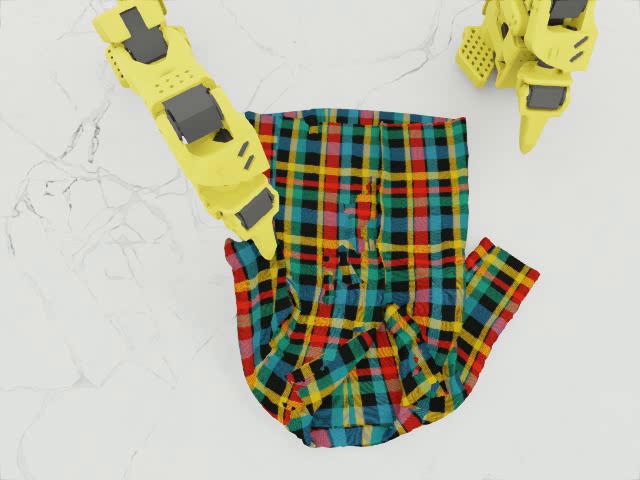
\includegraphics[width=0.12\textwidth]{fig/qualitative/ts_failure_1.png} &
        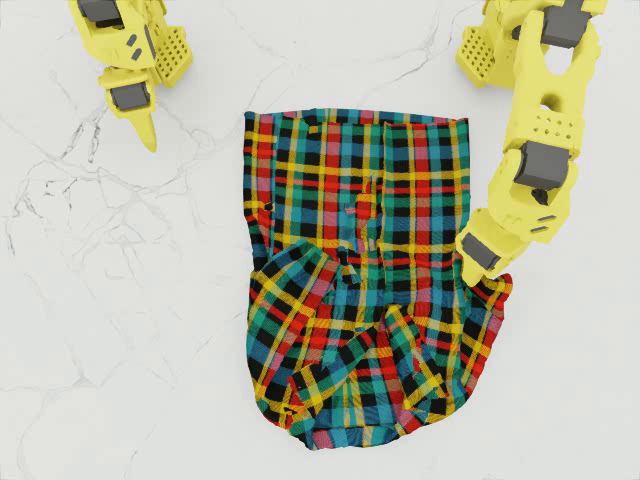
\includegraphics[width=0.12\textwidth]{fig/qualitative/ts_failure_2.png} &
        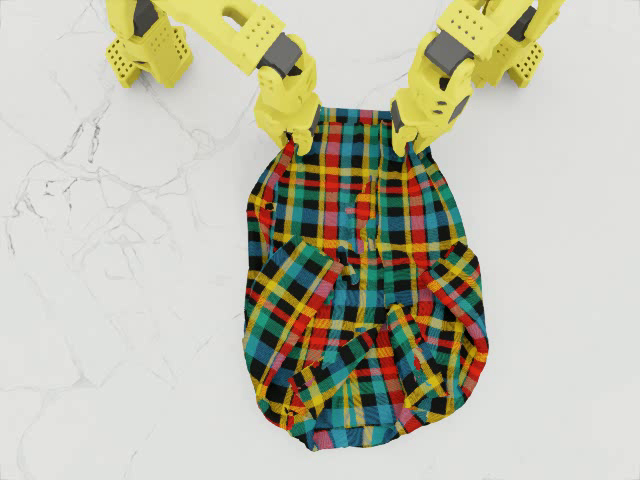
\includegraphics[width=0.12\textwidth]{fig/qualitative/ts_failure_3.png} &
        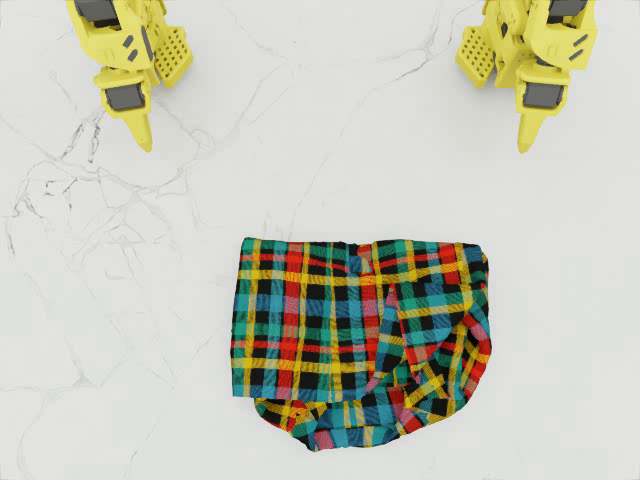
\includegraphics[width=0.12\textwidth]{fig/qualitative/ts_failure_4.png} &
        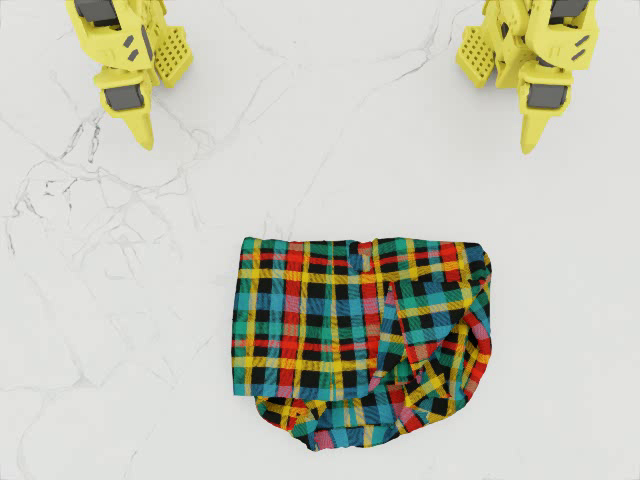
\includegraphics[width=0.12\textwidth]{fig/qualitative/ts_failure_5.png} &
        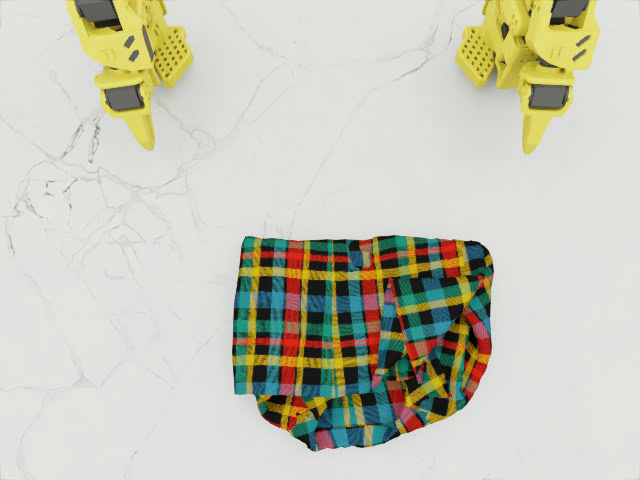
\includegraphics[width=0.12\textwidth]{fig/qualitative/ts_failure_6.png} &
        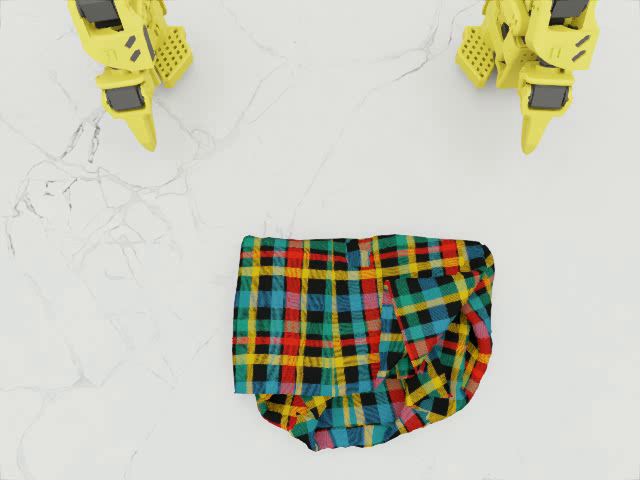
\includegraphics[width=0.12\textwidth]{fig/qualitative/ts_failure_7.png} \\
        \tiny $t=0.0s$ & \tiny $t=2.8s$ & \tiny $t=5.6s$ & \tiny $t=8.4s$ & \tiny $t=11.2s$ & \tiny $t=14.0s$ & \tiny $t=16.8s$ & \tiny $t=19.6s$ \\
        \multicolumn{8}{c}{\small (c) T-shirt Failure Mode} \\
    \end{tabular}
    \caption{Qualitative evaluation of our best ACT configuration across different garment categories. Rows 1 and 2 demonstrate successful bimanual folding of a long-sleeved top and long pants, respectively, showcasing robust coordination and trajectory planning with explicit timesteps ($t$). Row 3 illustrates a typical failure mode on a T-shirt; the model successfully initiates the fold but fails to properly release the garment's corner, leading to a timeout at 20 seconds.}
    \label{fig:qualitative_results}
\end{figure*}

\begin{itemize}[leftmargin=*,noitemsep]
    \item \textbf{SmolVLA Variants}: The base SmolVLA model performed significantly better than DP. As discussed in Section \ref{sec:ablation_aug}, the addition of PEFT (LoRA) further improved performance to 53.75\% on local evaluation. Notably, this model achieved a macro-average success rate of 49.50\% on the official competition leaderboard (20 garments per category; 80 total). However, as analyzed in Section \ref{sec:generalization}, PEFT showed signs of overfitting on unseen garments.
\end{itemize}

\subsection{Action Chunking with Transformers (ACT)}
Our final phase focused on ACT. As seen in Table \ref{tab:per_garment_results}, even the base ACT (58.96\%) outperformed the most optimized VLA configurations. ACT's ability to model action sequences as chunks effectively captured the temporal correlations between the two arms. Our final submission to the LeHome Challenge leaderboard is the \textbf{ACT + Depth + Aug + $n_{action}=1$} configuration (ResNet backbone); while official results for this specific submission are currently pending, its local performance (62.92\%) and generalization (51.25\%) suggest high competitive potential.

\subsection{Ablation and Sensitivity Analysis}
\label{sec:ablation}
We perform a detailed ablation study to isolate the impact of our architectural choices.

\subsubsection{Backbone Comparison: ResNet vs. DINOv2}
Replacing the ResNet-18 backbone with DINOv2 resulted in our best "seen" macro-average of 63.54\%. However, as shown in Table \ref{tab:unseen_per_garment}, this performance gain did not fully translate to unseen garments (43.75\%), suggesting that the high-capacity DINOv2 features may be more susceptible to appearance-based overfitting on our 80-trajectory dataset.

\subsubsection{Impact of Data Augmentation and PEFT}
\label{sec:ablation_aug}
We investigated the relative contributions of stochastic augmentations and Parameter-Efficient Fine-Tuning (PEFT). 
\begin{itemize}[leftmargin=*,noitemsep]
    \item \textbf{Stochastic Augmentations}: Applying random cropping and rotation to the SmolVLA model improved the local success rate. More importantly, it was the primary driver of generalization, allowing the model to achieve 50.00\% on unseen garments.
    \item \textbf{PEFT via LoRA}: While LoRA-based fine-tuning boosted performance on seen garments (53.75\%), it led to a significant drop on unseen garments (25.00\%). This highlights a critical trade-off in VLA adaptation: fine-tuning massive backbones on limited task-specific data can degrade the model's inherent zero-shot capabilities.
\end{itemize}

\subsubsection{Chunk Size and Temporal Parameters}
We compared chunk sizes ($k$) of 64, 100, and 128. As shown in Table \ref{tab:per_garment_results}, $k=100$ provided the best balance between trajectory smoothness and reactivity. 

\subsection{Generalization to Unseen Garments}
\label{sec:generalization}
We evaluate the robustness of all configurations on a hold-out set of 2 unseen garments per category. Table \ref{tab:unseen_per_garment} presents the exhaustive results across all 12 evaluated models.

\begin{table*}[t]
\centering
\caption{Exhaustive per-garment success rates (\%) on unseen garment styles across all evaluated architectures. Hyphen (-) indicates configurations not evaluated for that category due to baseline failure.}
\label{tab:unseen_per_garment}
\resizebox{\textwidth}{!}{%
\begin{tabular}{lccccc}
\toprule
\textbf{Model Configuration} & \textbf{T-L (\%)} & \textbf{T-S (\%)} & \textbf{P-L (\%)} & \textbf{P-S (\%)} & \textbf{Macro-Avg (\%)} \\
\midrule
Diffusion Policy (DP)$^\ast$ & 5.00\% & 0.00\% & 3.00\% & 38.33\% & 11.58\% \\
SmolVLA (Base) & 30.00\% & 0.00\% & 20.00\% & 60.00\% & 27.50\% \\
SmolVLA + Aug & 60.00\% & 30.00\% & 70.00\% & 40.00\% & 50.00\% \\
SmolVLA + Aug + PEFT (LoRA) & 50.00\% & 0.00\% & 25.00\% & 25.00\% & 25.00\% \\
\midrule
$\pi_{0.5}$ (Base) & - & 0.00\% & 0.00\% & - & 0.00\% \\
$\pi_{0.5}$ + PEFT (LoRA) & - & 0.00\% & 0.00\% & - & 0.00\% \\
X-VLA + PEFT (LoRA) & - & 0.00\% & - & - & 0.00\% \\
\midrule
ACT (Base) & 85.00\% & 30.00\% & 30.00\% & 45.00\% & 47.50\% \\
ACT + Depth & 60.00\% & 35.00\% & 10.00\% & 55.00\% & 40.00\% \\
ACT + Depth + Aug (Chunk 64) & - & 5.00\% & 40.00\% & - & 11.25\% \\
ACT + Depth + Aug (Chunk 100) & 45.00\% & 35.00\% & 70.00\% & 55.00\% & 51.25\% \\
ACT + Depth + Aug (Chunk 128) & 60.00\% & 30.00\% & 65.00\% & 45.00\% & 50.00\% \\
\textbf{ACT + Depth + Aug + $n_{action}=1$} & \textbf{70.00\%} & \textbf{15.00\%} & \textbf{75.00\%} & \textbf{45.00\%} & \textbf{51.25\%} \\
ACT + Depth + Aug + $n_{action}=1$ + DINOv2 & 50.00\% & 15.00\% & 55.00\% & 55.00\% & 43.75\% \\
\bottomrule
\multicolumn{6}{l}{$^\ast$ Evaluated on 5 episodes per garment category; all other models evaluated on 10 episodes.} \\
\end{tabular}%
}
\end{table*}

The comparison reveals that while the DINOv2 backbone and PEFT adapters improve performance on seen data, simpler architectures with heavy augmentations often provide more robust generalization. Interestingly, we observe that the introduction of depth information in isolation (\textit{ACT + Depth}) led to a decrease in generalization (40.00\%) compared to the base model (47.50\%). Given the significant generalization gains observed when applying augmentations to our VLA baseline (Section \ref{sec:ablation_aug}), this result suggests that the rich geometric features provided by depth maps are particularly susceptible to overfitting on the specific topography and wrinkle patterns of the training garments. This underscores the necessity of combining high-dimensional multimodal inputs with robust regularization strategies like stochastic data augmentation to achieve stable generalization. 

Our final submission (\textbf{ResNet-based ACT}) achieves a superior balance, matching the highest unseen macro-average of 51.25\% while maintaining strong performance across both tops and pants.

\subsection{Limitations and Future Work}
\label{sec:limitations}
Our study was significantly impacted by both infrastructure and algorithmic constraints. Infrastructurally, we utilized a shared HPC environment with an NVIDIA RTX 4090 (24GB), which was often unavailable, leading to substantial delays. Algorithmically, the policy is currently bottlenecked by the "expert-only" nature of the training dataset. Since the provided trajectories consist exclusively of successful teleoperated demonstrations, the model never observes the transitions required to recover from stochastic failures (e.g., losing contact with a cloth corner). Furthermore, the lack of a graphical interface on the HPC prevented the implementation of online corrective frameworks like DAgger, as real-time visual feedback for corrective demonstrations was not feasible.

Future research will focus on implementing online corrective feedback to address the distribution shift inherent in behavioral cloning. We also plan to explore combining the strengths of transformer-based action chunking with the vast pre-trained knowledge of VLAs by using foundation models as visual encoders for ACT. Additionally, we aim to extend this framework to multi-task scenarios and more complex robotic embodiments, where the data efficiency of ACT and the semantic understanding of VLAs can be combined for more capable manipulation systems.

    